\subsection{Introduction}
The burst analysis procedures generate a series of parameters representative for
each burst. The most commonly employed parameters are listed in the following:
\begin{itemize}
    \item Percentage of bursting channels
    \item Total number of bursts
    \item Mean bursting rate (\(MBR\), expressed in \(bursts/min\))
    \item Burst duration
    \item Inter burst interval (\(IBI\)) - it can be either start-to-start (not
    influenced by burst duration) or end-to-start
    \item Total number of spikes in a bursting channel
    \item Percentage of random spikes
    \item Mean intra-burst frequency
    \item Peak intra-burst frequency
\end{itemize}
Notice that sometimes it might be useful also to evaluate the out-burst spikes.

\subsection{Data visualization tools}
In the following there is a detailed description of the main tools to characterize and
visualize bursting activity.

\subsubsection{Inter Burst Interval}
The inter burst interval (\(IBI\)) represents the burst equivalent of \(ISI\) for
the spikes. Also in the case of \(IBI\) it is possible to plot an histogram,
denominated \(IBIH\). Burst are defined as macro events with a specific duration,
however it becomes less and less relevant as the recording period is increased.
Thus, under the hypothesis of long term recordings (in the order of tens of minutes)
it is possible to consider burst events as single-point events, exactly as it is done
for spikes. The mathematical formulation of the inter burst interval is given below:
\begin{align*}
    IBIH(\tau)=\frac{1}{M-1}\sum_{b=1}^{M-1}\delta(t_{b+1}-t_{b}-\tau)
\end{align*}
with \(M\) being the total number of burst events.
In a similar fashion, the analogous concepts of JIBI (Joint IBI) and CIBI (Cross IBI)
can be defined.
\begin{figure}[H]
    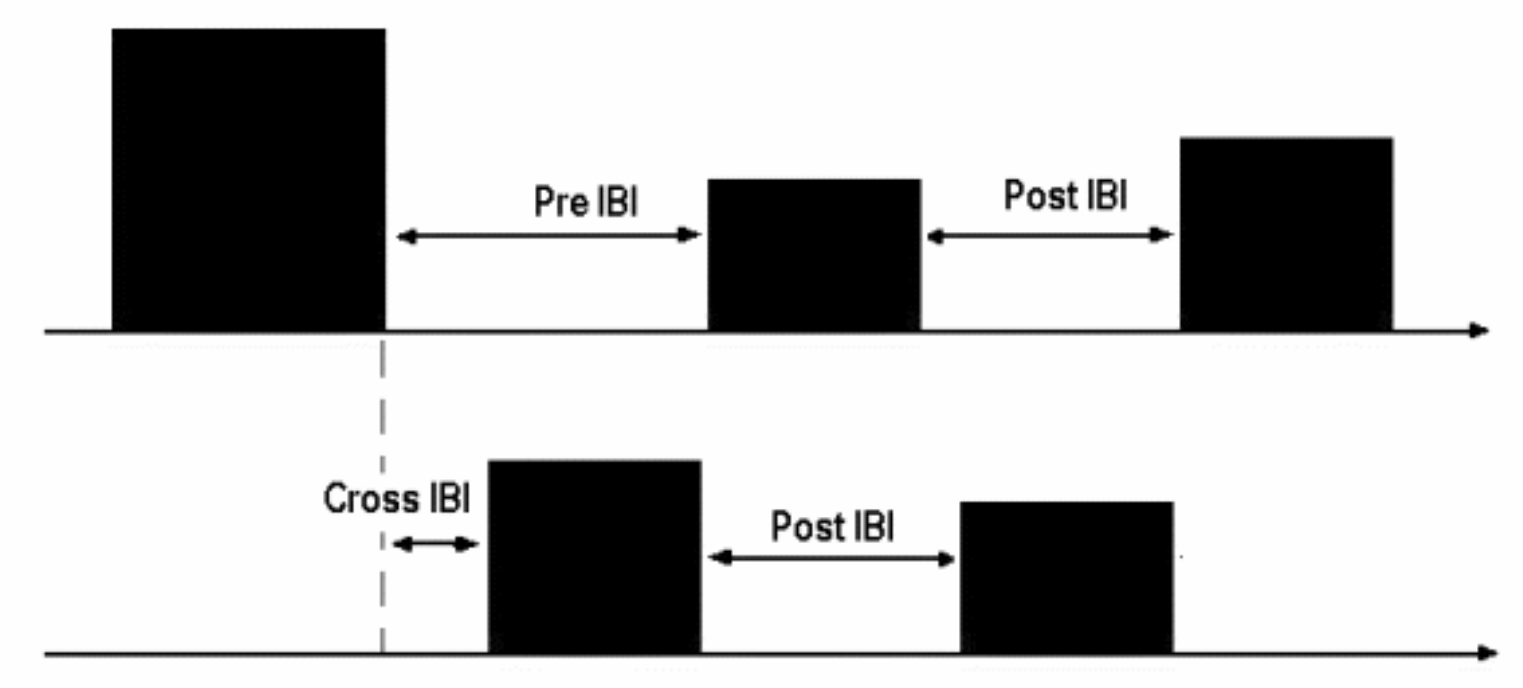
\includegraphics[scale=0.28]{6_1}
    \centering
\end{figure}

\subsubsection{Fano Factor and Coefficient of Variation}
The Fano Factor (\(FF\)) dispersion is a reliable measure of the variability of events
(either spikes or bursts) across a given population. The \(FF\) dispersion is
immediately obtained by computing the average number of events \(\langle{N(T)}\rangle\)
in a time interval \(T\) (thus for each bin), together with its corresponding variance
\(Var\{N(T)\}\), as displayed in the following expression:
\begin{align*}
    FF(T)=\frac{Var\{N(T)\}}{\langle{N(T)}\rangle}
\end{align*}
On the other hand, by replacing the variance with the standard deviation
\(\sigma\bigl[N(T)\bigr]\), one could compute the Coefficient of Variation
\(CV\):
\begin{align*}
    CV(T)=\frac{\sigma\bigl[N(T)\bigr]}{\langle{N(T)}\rangle}
\end{align*}
Notice that the Coefficient of Variation defined here is exactly the same
measure defined some pages above, denoted as \(C_v\).

\subsubsection{State Space Plot}
This type of representation visualizes data points as function of burst duration
and burst number (or alternatively burst rate). State space plots are
especially valuable to compare the activity of different channels or different
subjects, as they tend to point out differences in the bursts distribution,
for instance they might be used to show the different activity between two
subjects, one with a pathological condition and the other being totally healthy.
\begin{figure}[H]
    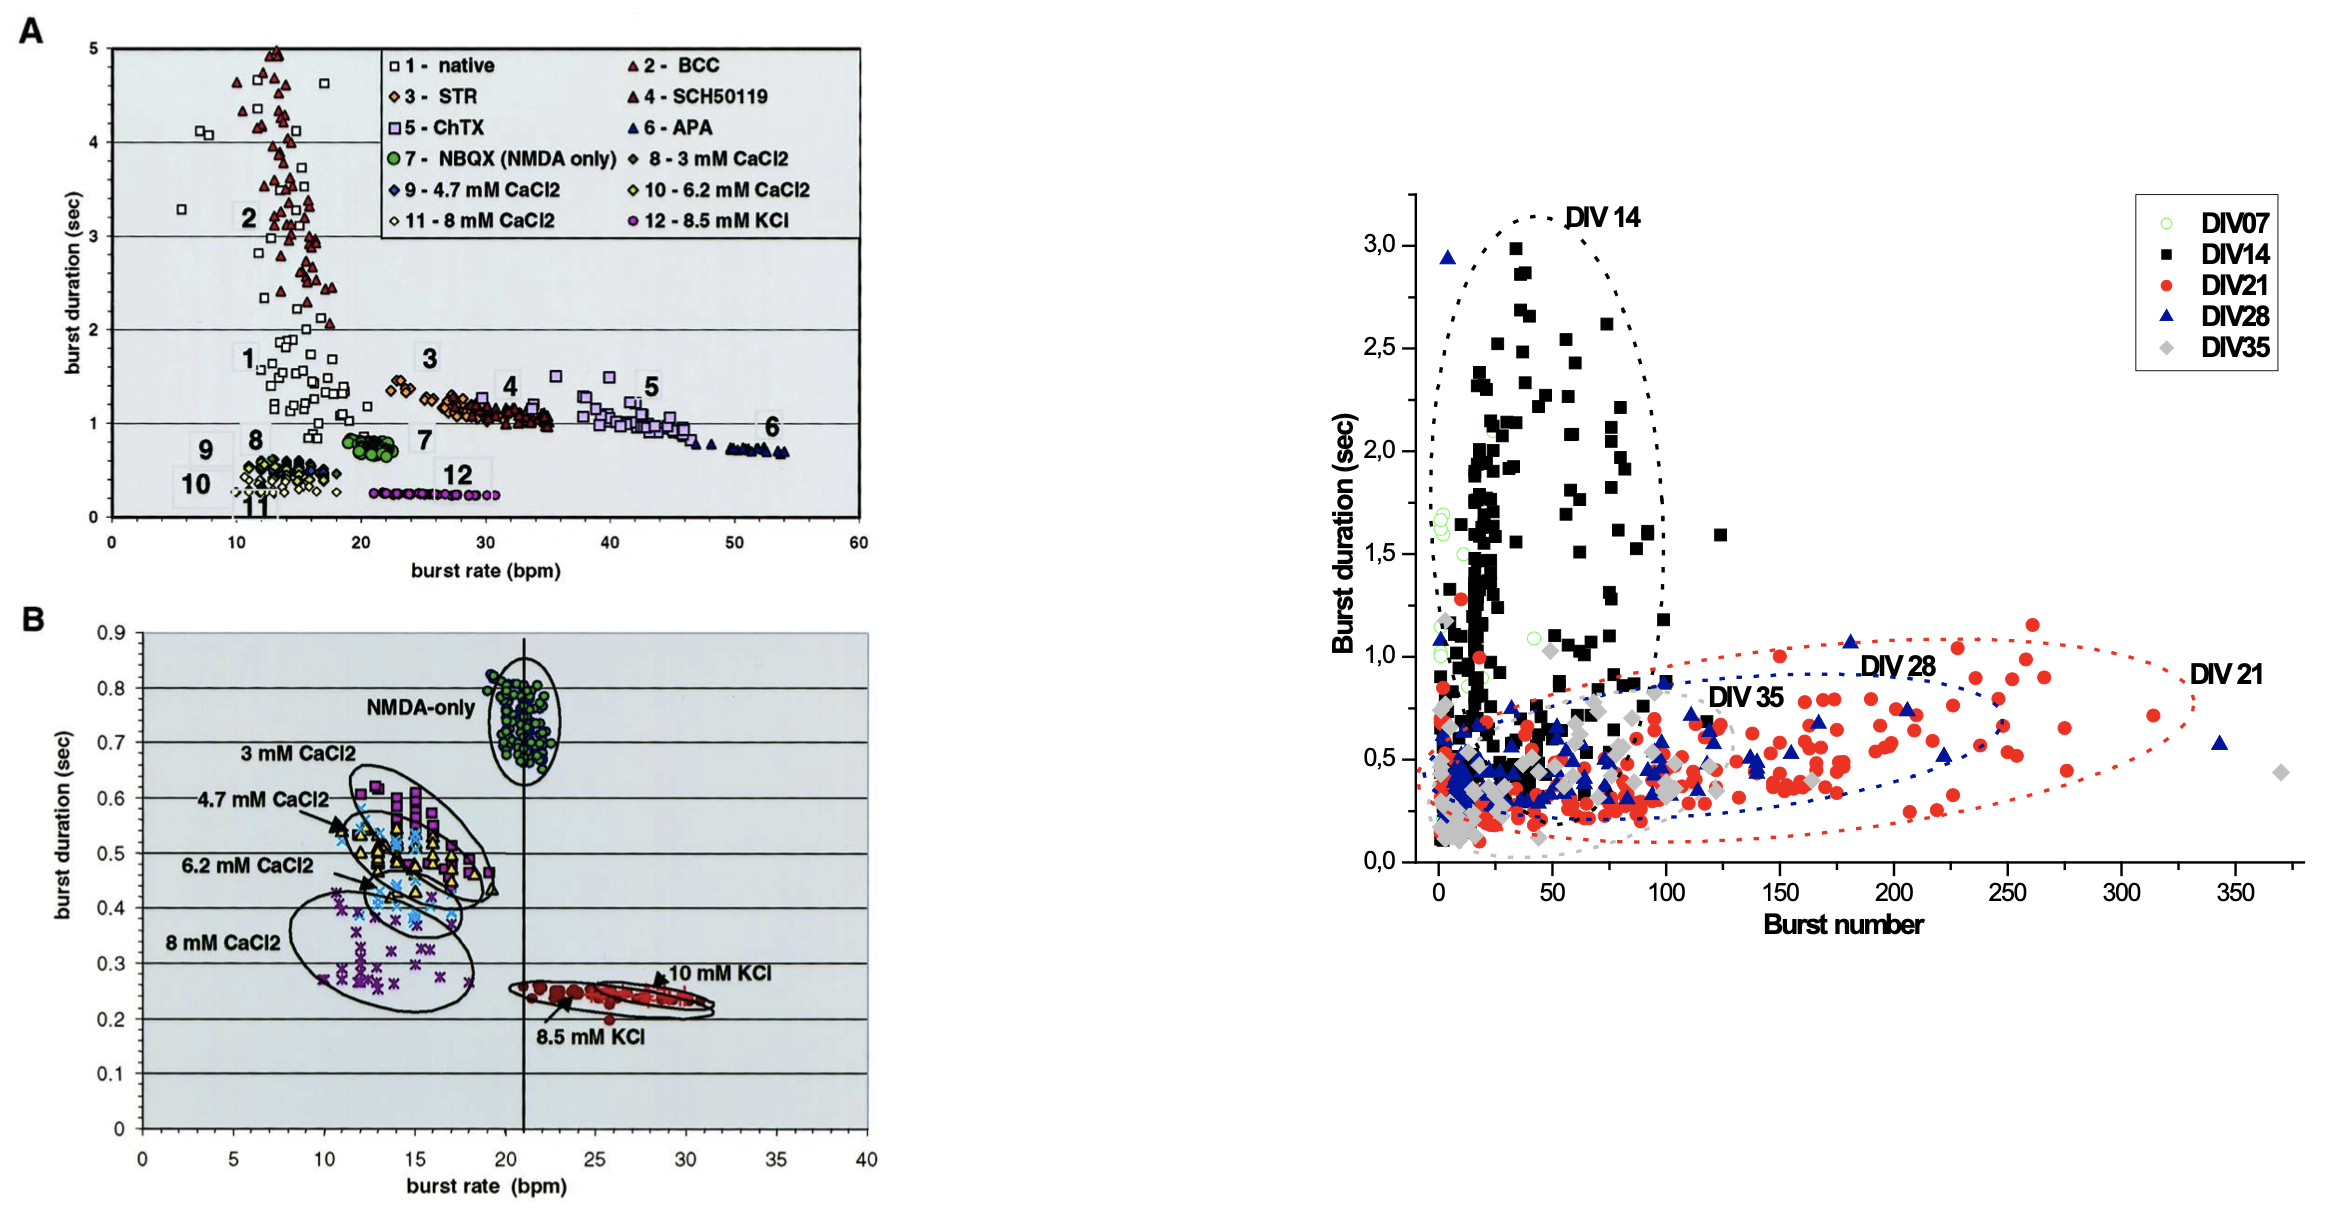
\includegraphics[scale=0.7]{6_2}
    \centering
\end{figure}